\documentclass{article}
\usepackage{style-lectures}
\usepackage{hyperref}					% setup internal and external links
\hypersetup{							% set up hyperlinks (used for toc here)
   hidelinks,								% hide links (don't change appearance of text that is clickable)
   linktoc=all    								% make toc clickable (all levels)
} % needs to be local

\title{MATH 321: Mathematical Statistics\\Completed Lectures}
\author{Colton Gearhart}
\date{\today}							

\begin{document}
\setcounter{secnumdepth}{0}		% trick to get unnumbered sections in table of contents
\maketitle
\dosecttoc
\tableofcontents
\newpage

%-------------------------------------------------------------------------
\section{Test 1}
%-------------------------------------------------------------------------

\secttoc

%----------------------------
\subsection{Lecture 14 -- Bivariate Distributions}
\includepdf[pages=-]{lecture-14-COMPLETED.pdf}\newpage
%----------------------------

%----------------------------
\subsection{Lecture 15 -- Conditional Distributions}
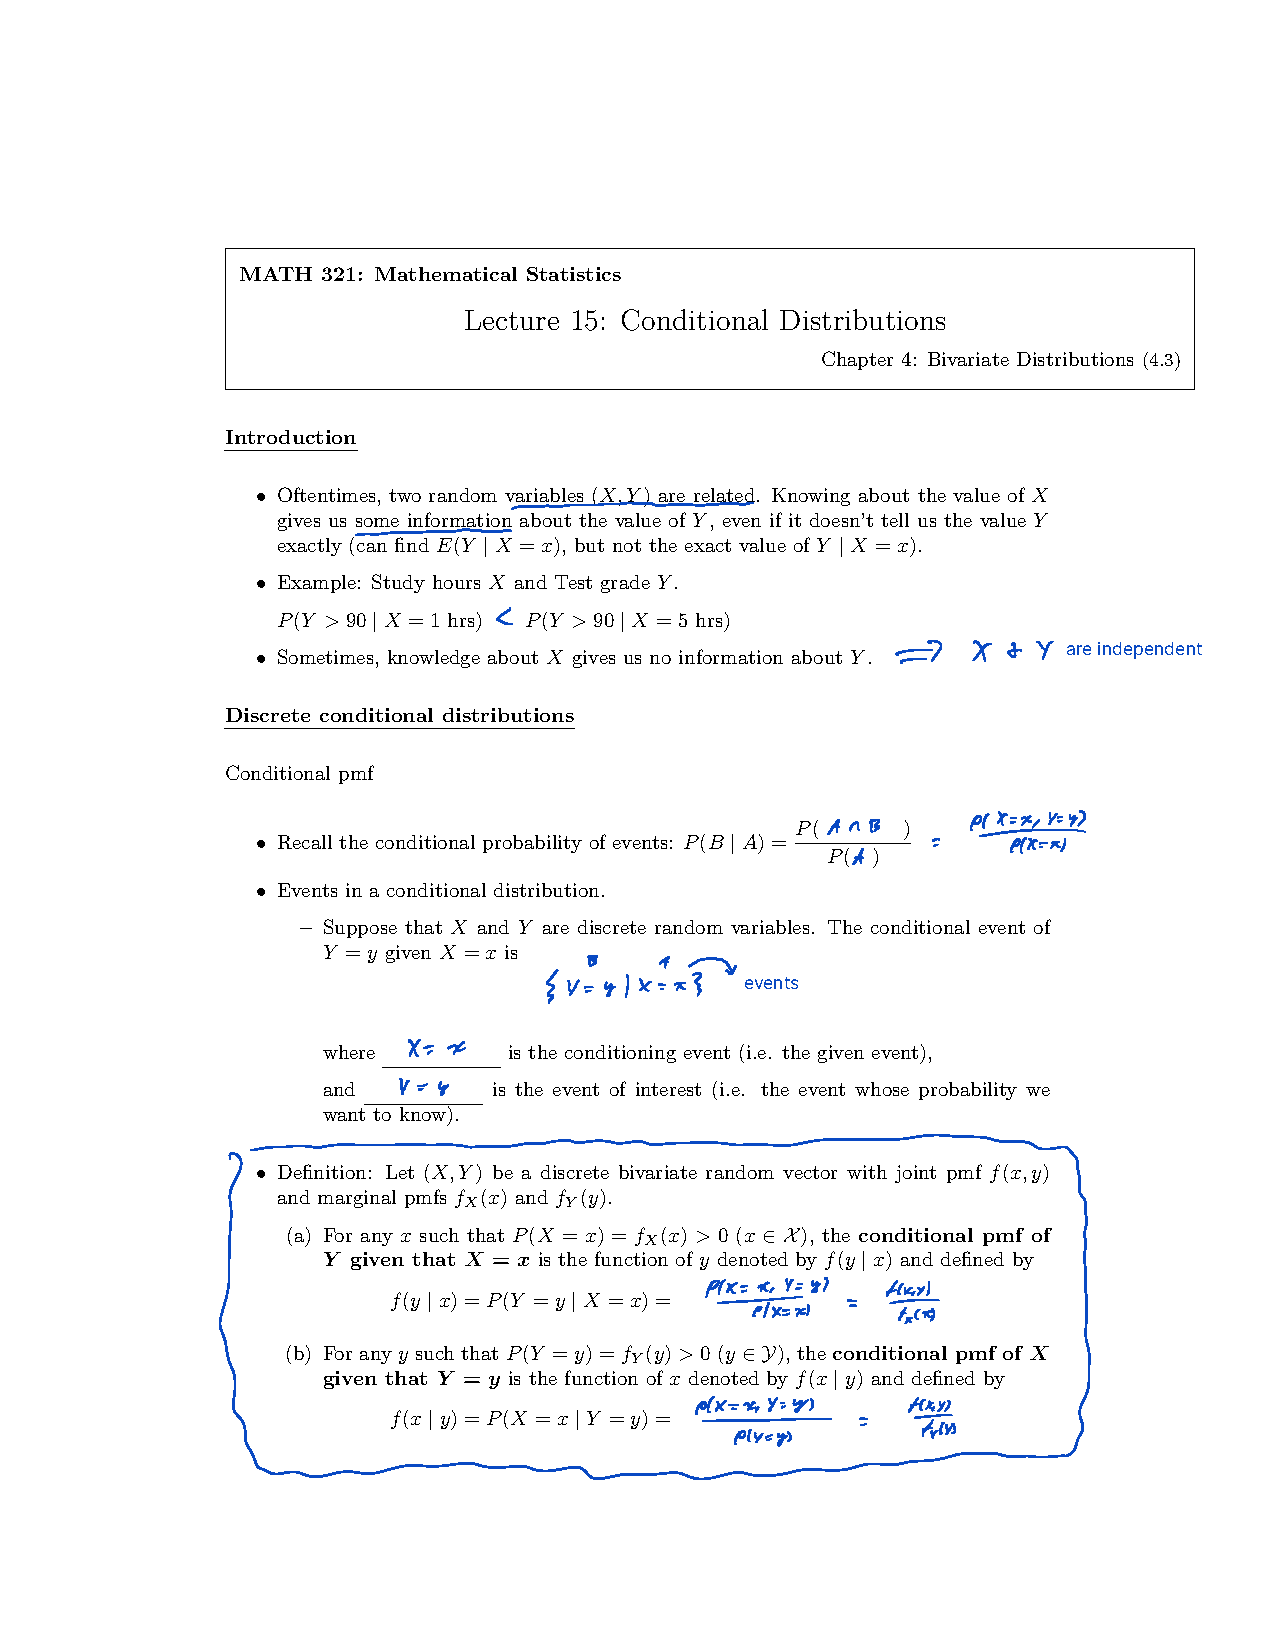
\includepdf[pages=-]{lecture-15-COMPLETED.pdf}\newpage
%----------------------------

%----------------------------
\subsection{Lecture 16 -- Independence and the Correlation Coefficient}
\includepdf[pages=-]{lecture-16-COMPLETED.pdf}\newpage
%----------------------------

%----------------------------
\subsection{Lecture 17 -- Several Random Variables}
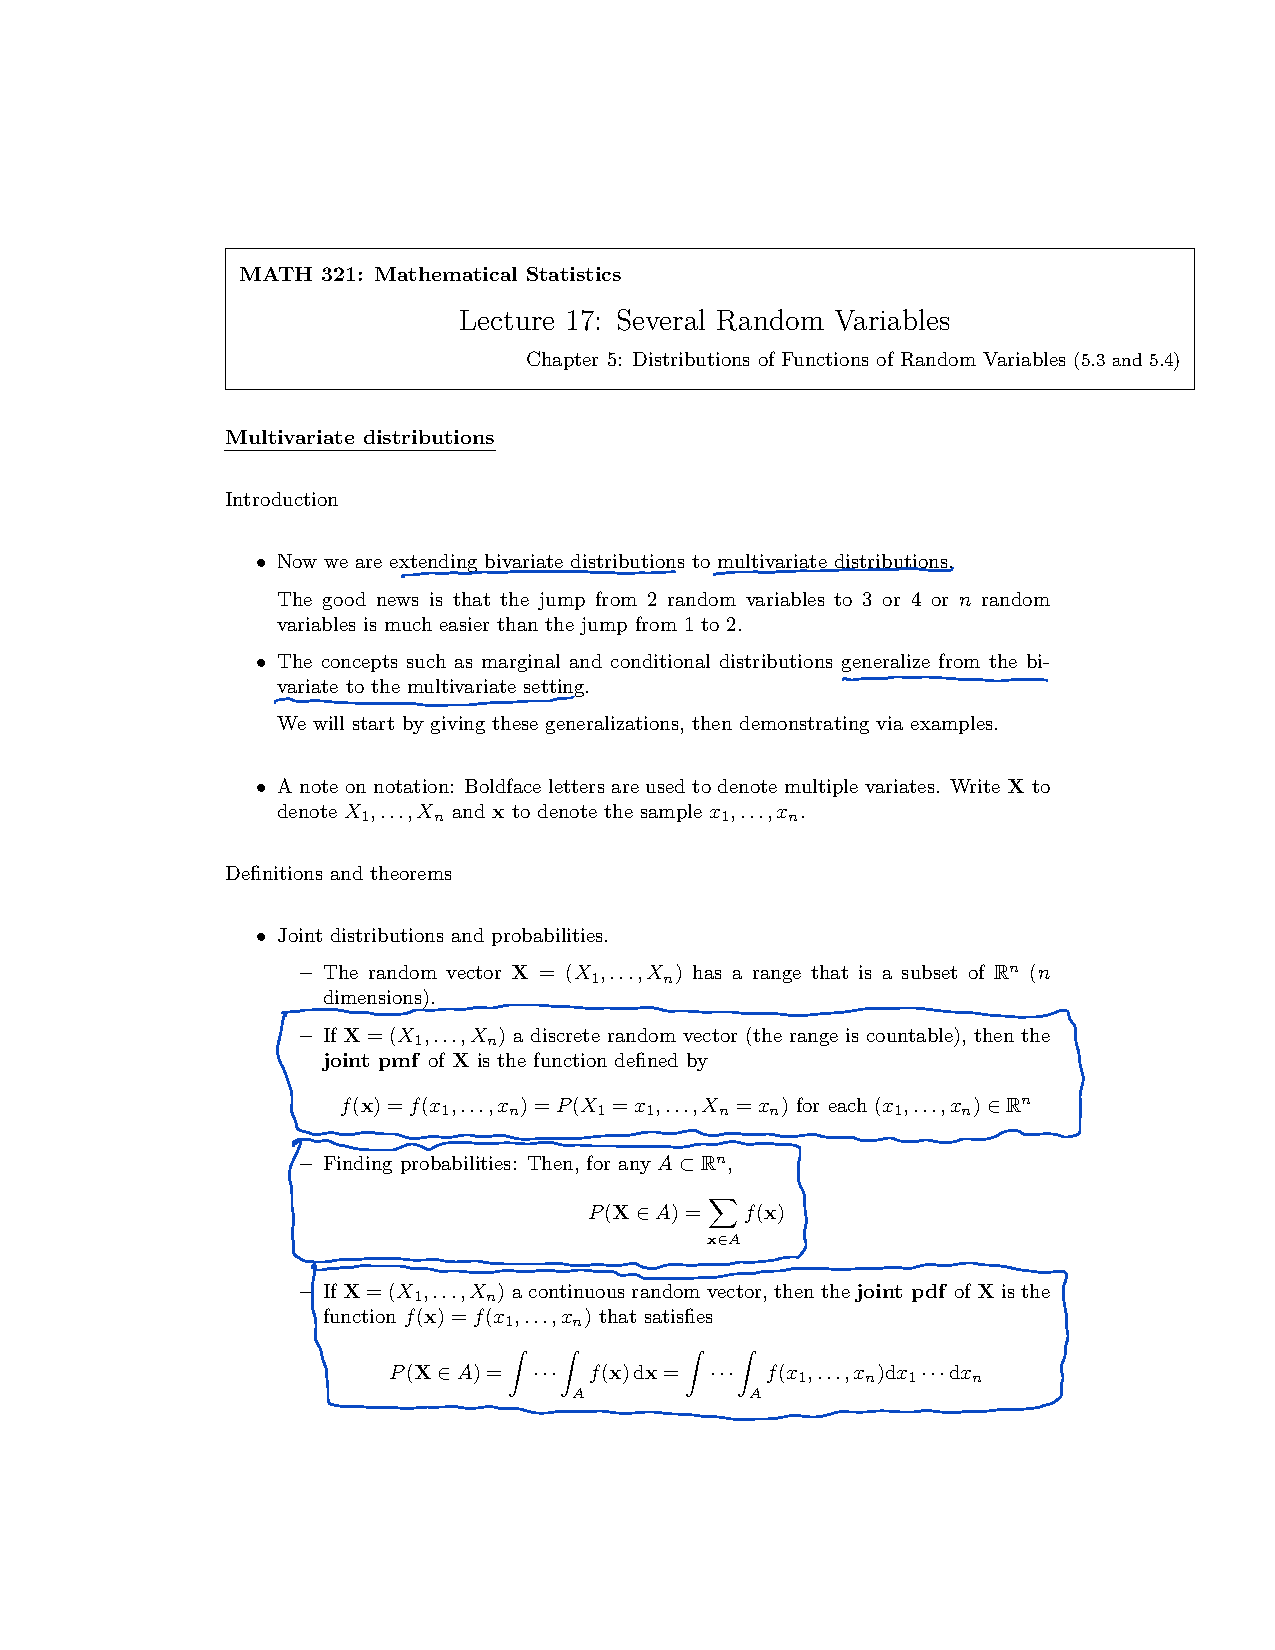
\includepdf[pages=-]{lecture-17-COMPLETED.pdf}\newpage
%----------------------------


%-------------------------------------------------------------------------
\section{Test 2}
%-------------------------------------------------------------------------

\secttoc

%----------------------------
\subsection{Lecture 1 -- Random Samples and Common Statistics}
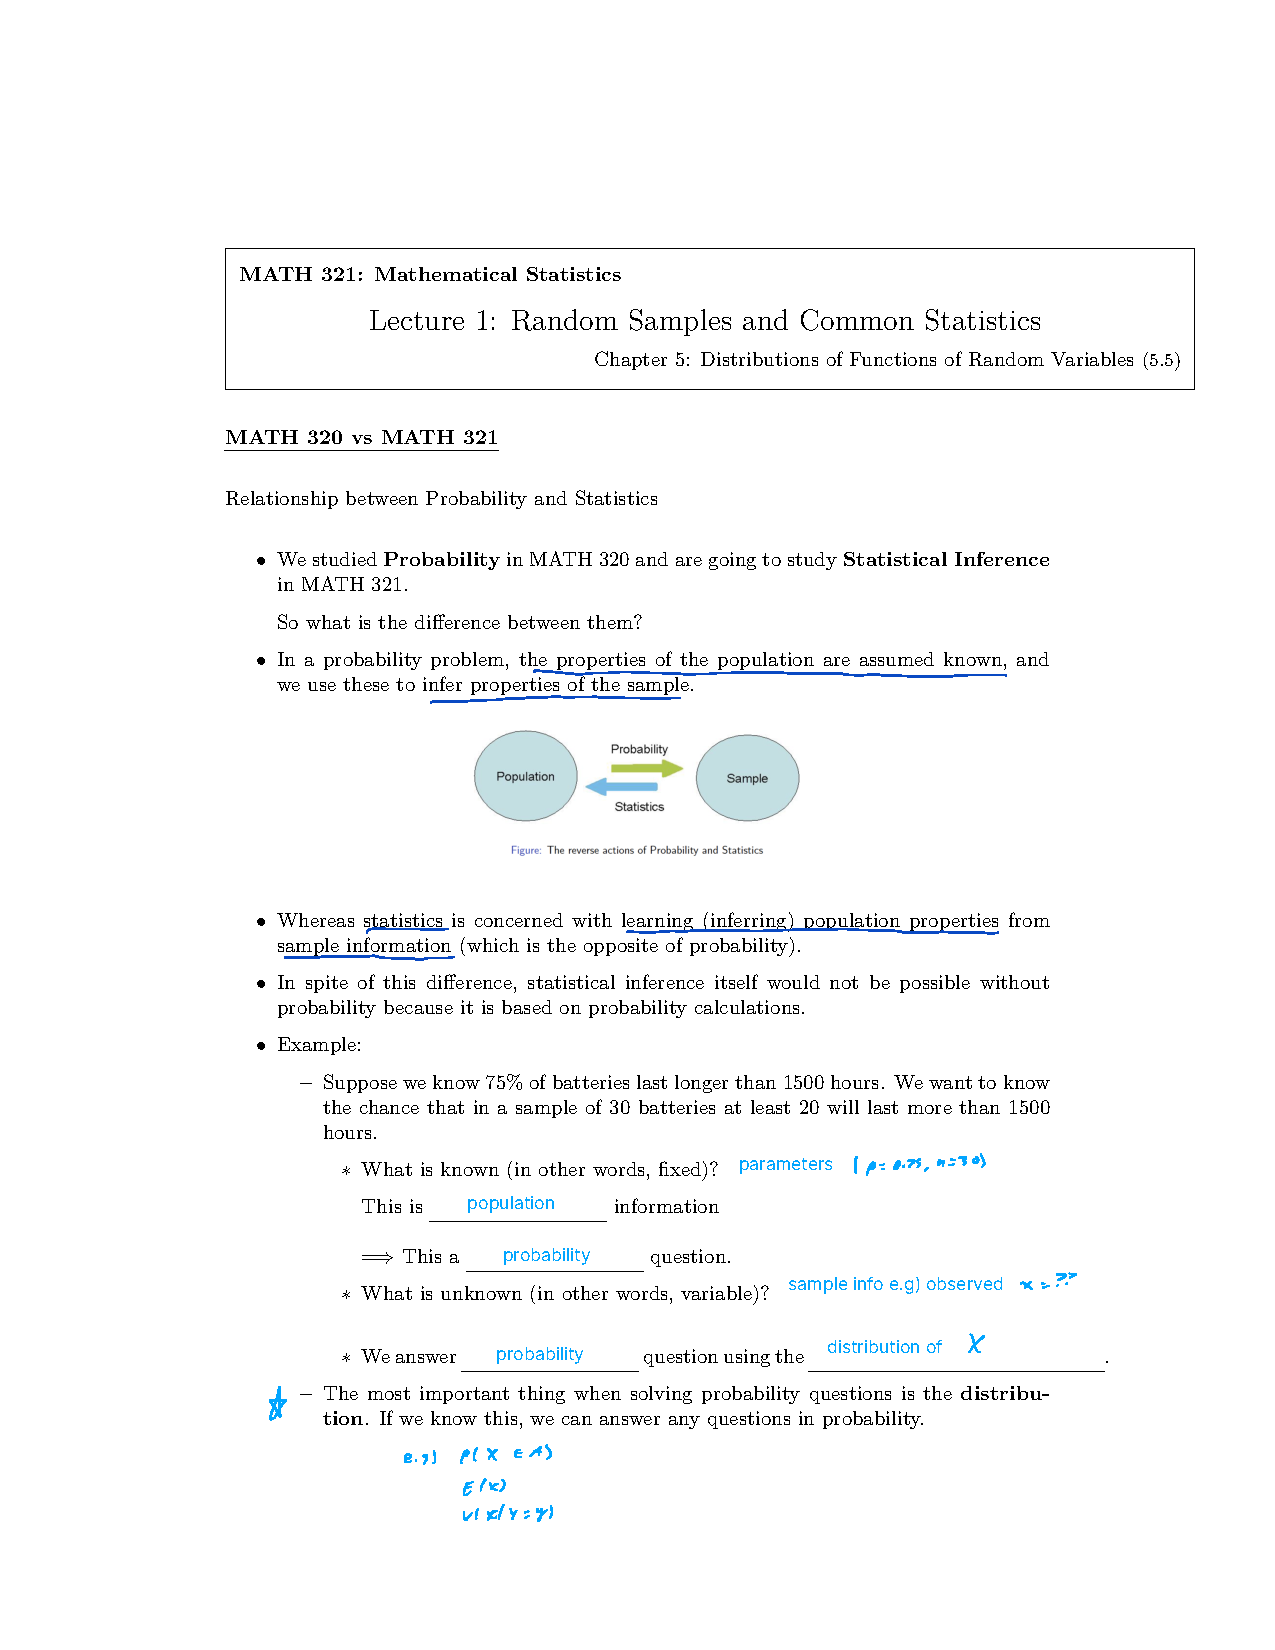
\includepdf[pages=-]{lecture-1-COMPLETED.pdf}\newpage
%----------------------------

%----------------------------
\subsection{Lecture 2 -- Order Statistics}
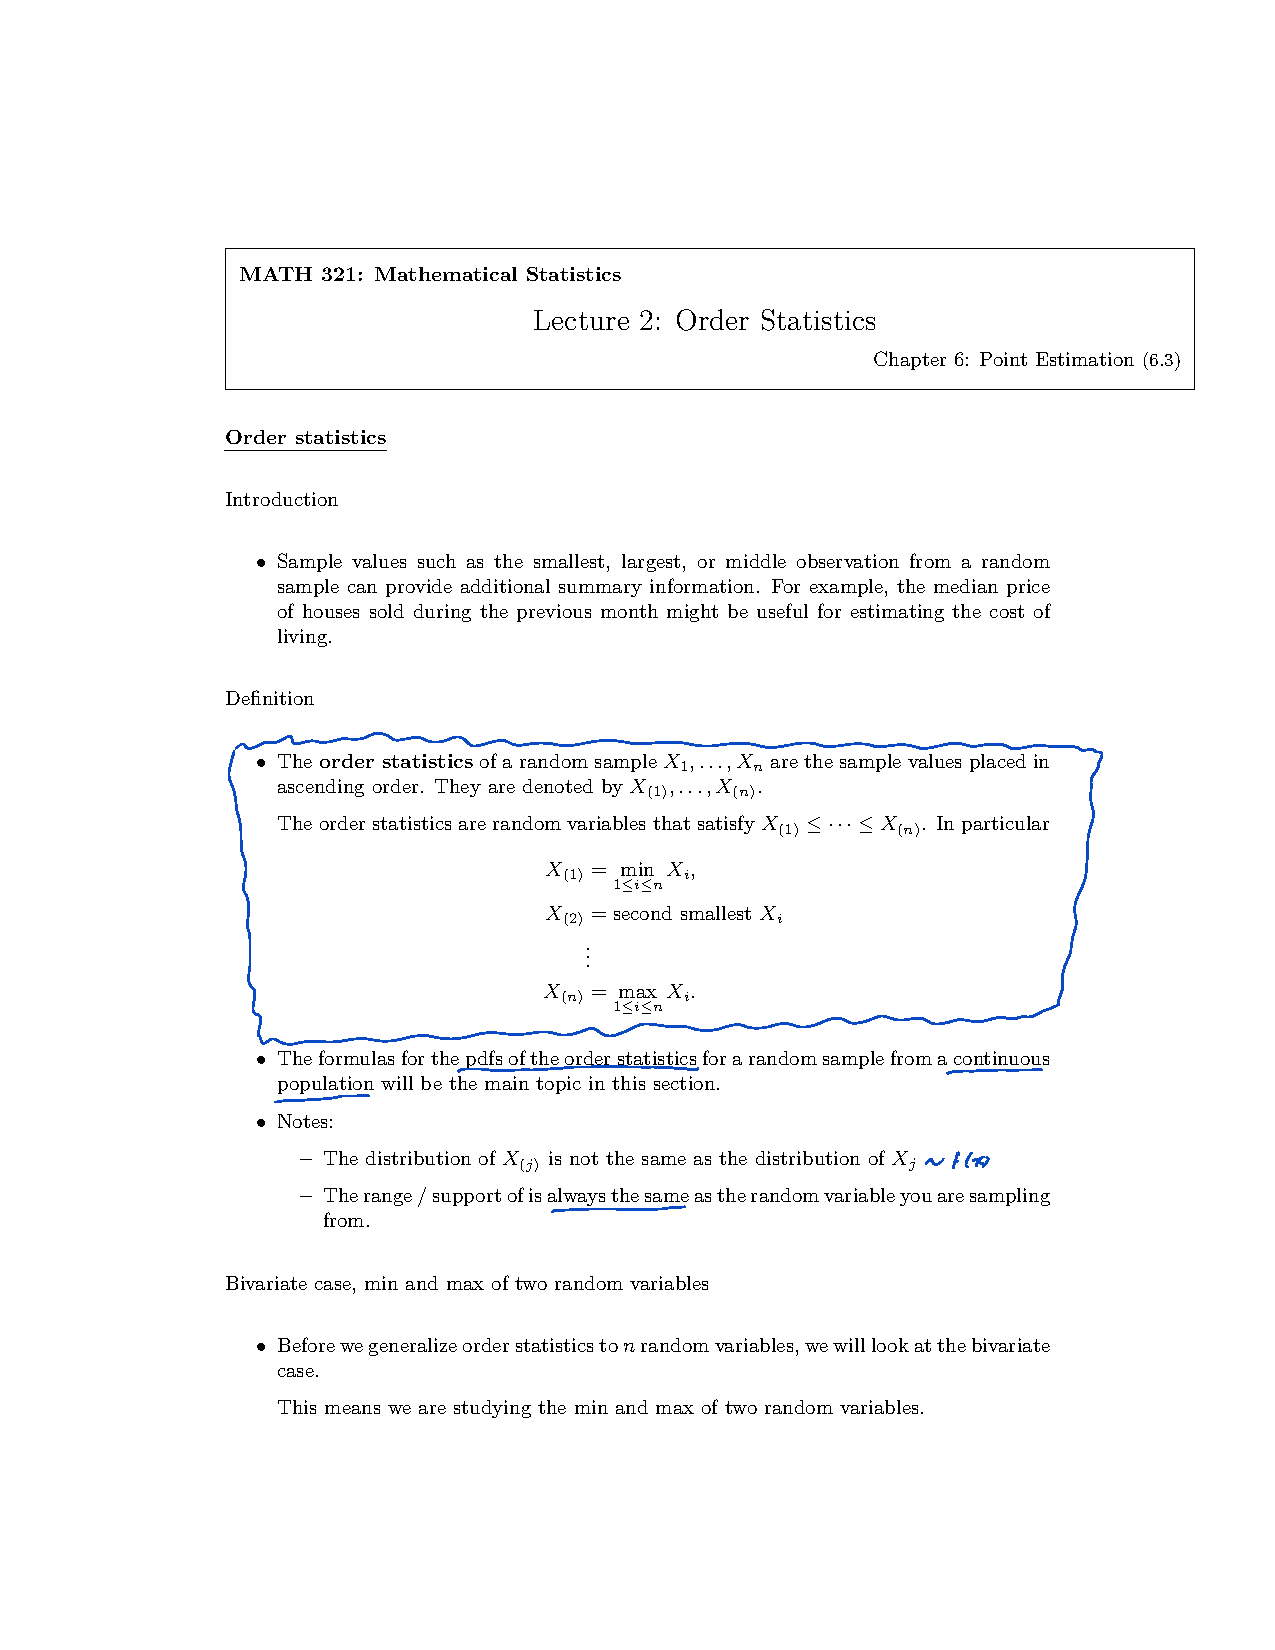
\includepdf[pages=-]{lecture-2-COMPLETED.pdf}\newpage
%----------------------------

%----------------------------
\subsection{Lecture 4 -- Point Estimation}
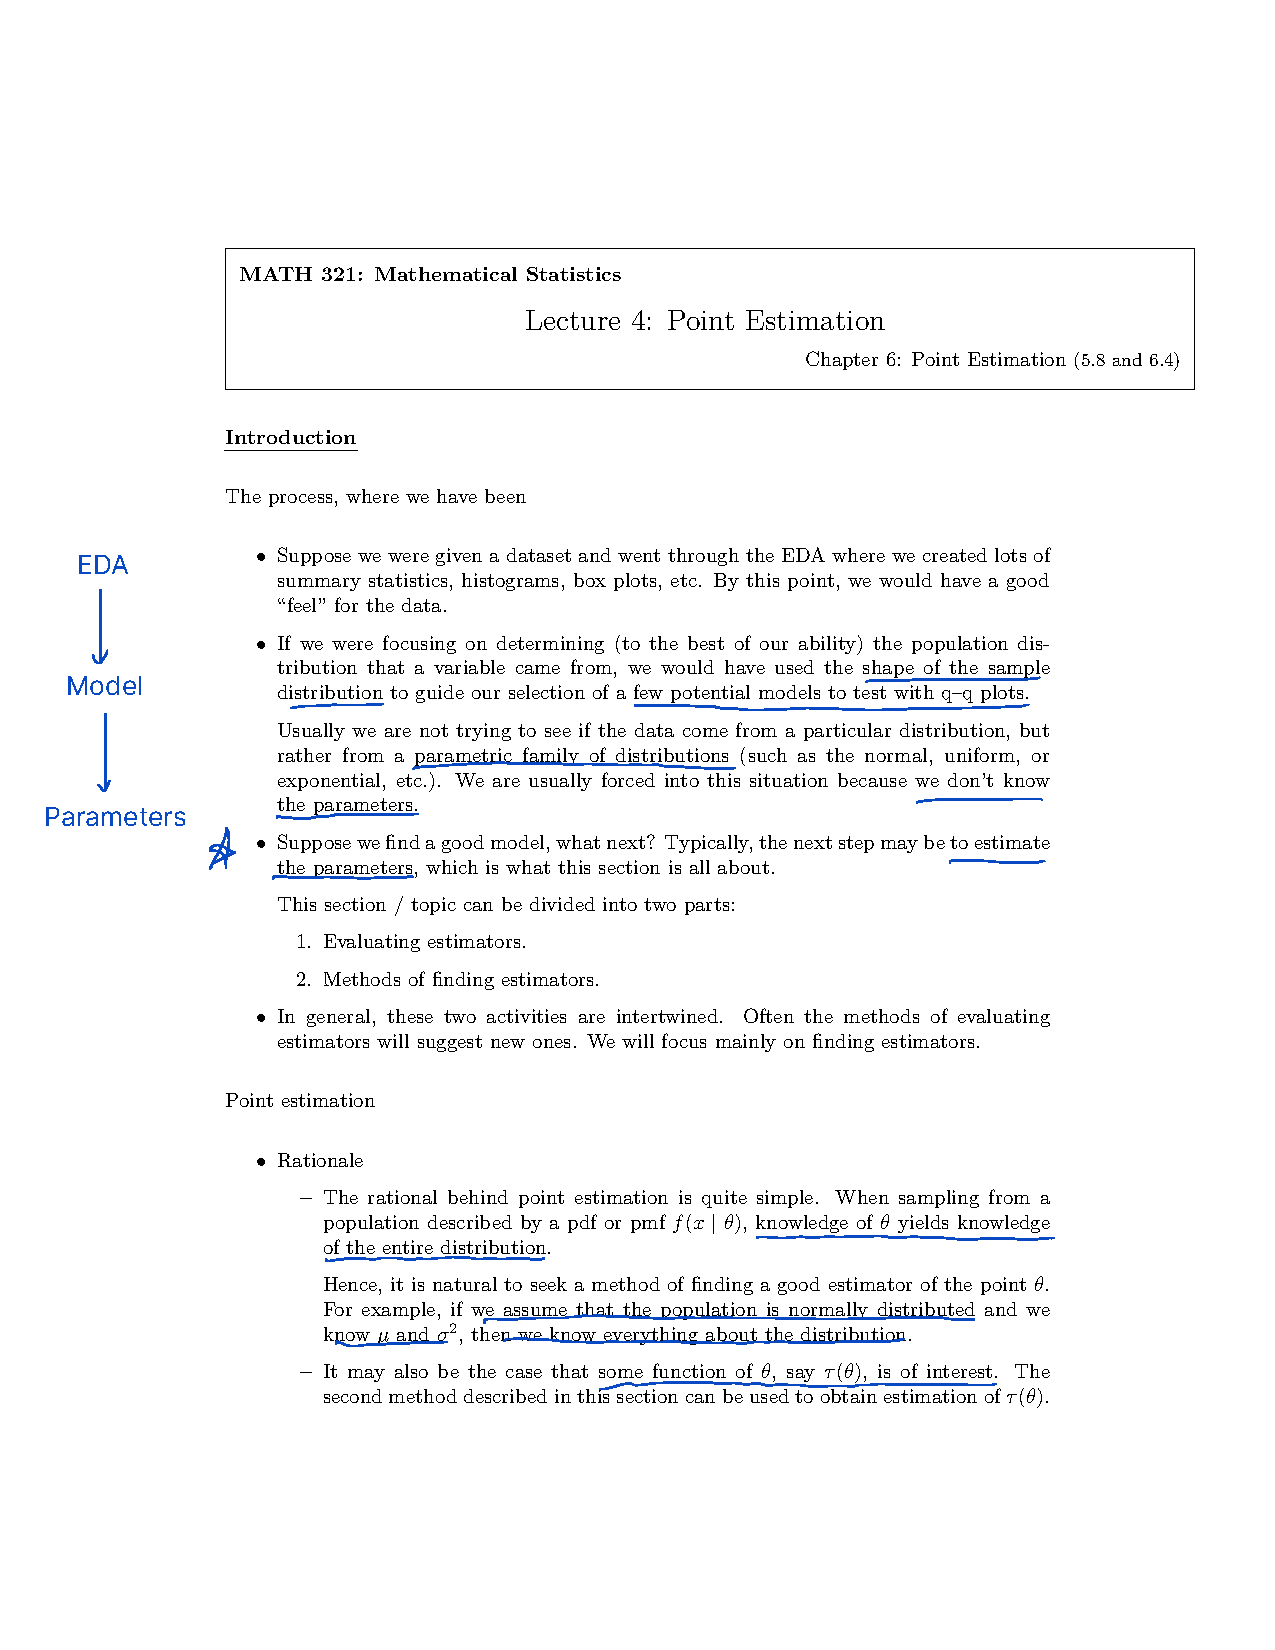
\includepdf[pages=-]{lecture-4-COMPLETED.pdf}\newpage
%----------------------------


%-------------------------------------------------------------------------
\section{Test 3}
%-------------------------------------------------------------------------

\secttoc

%----------------------------
\subsection{Lecture 5 -- The Central Limit Theorem}
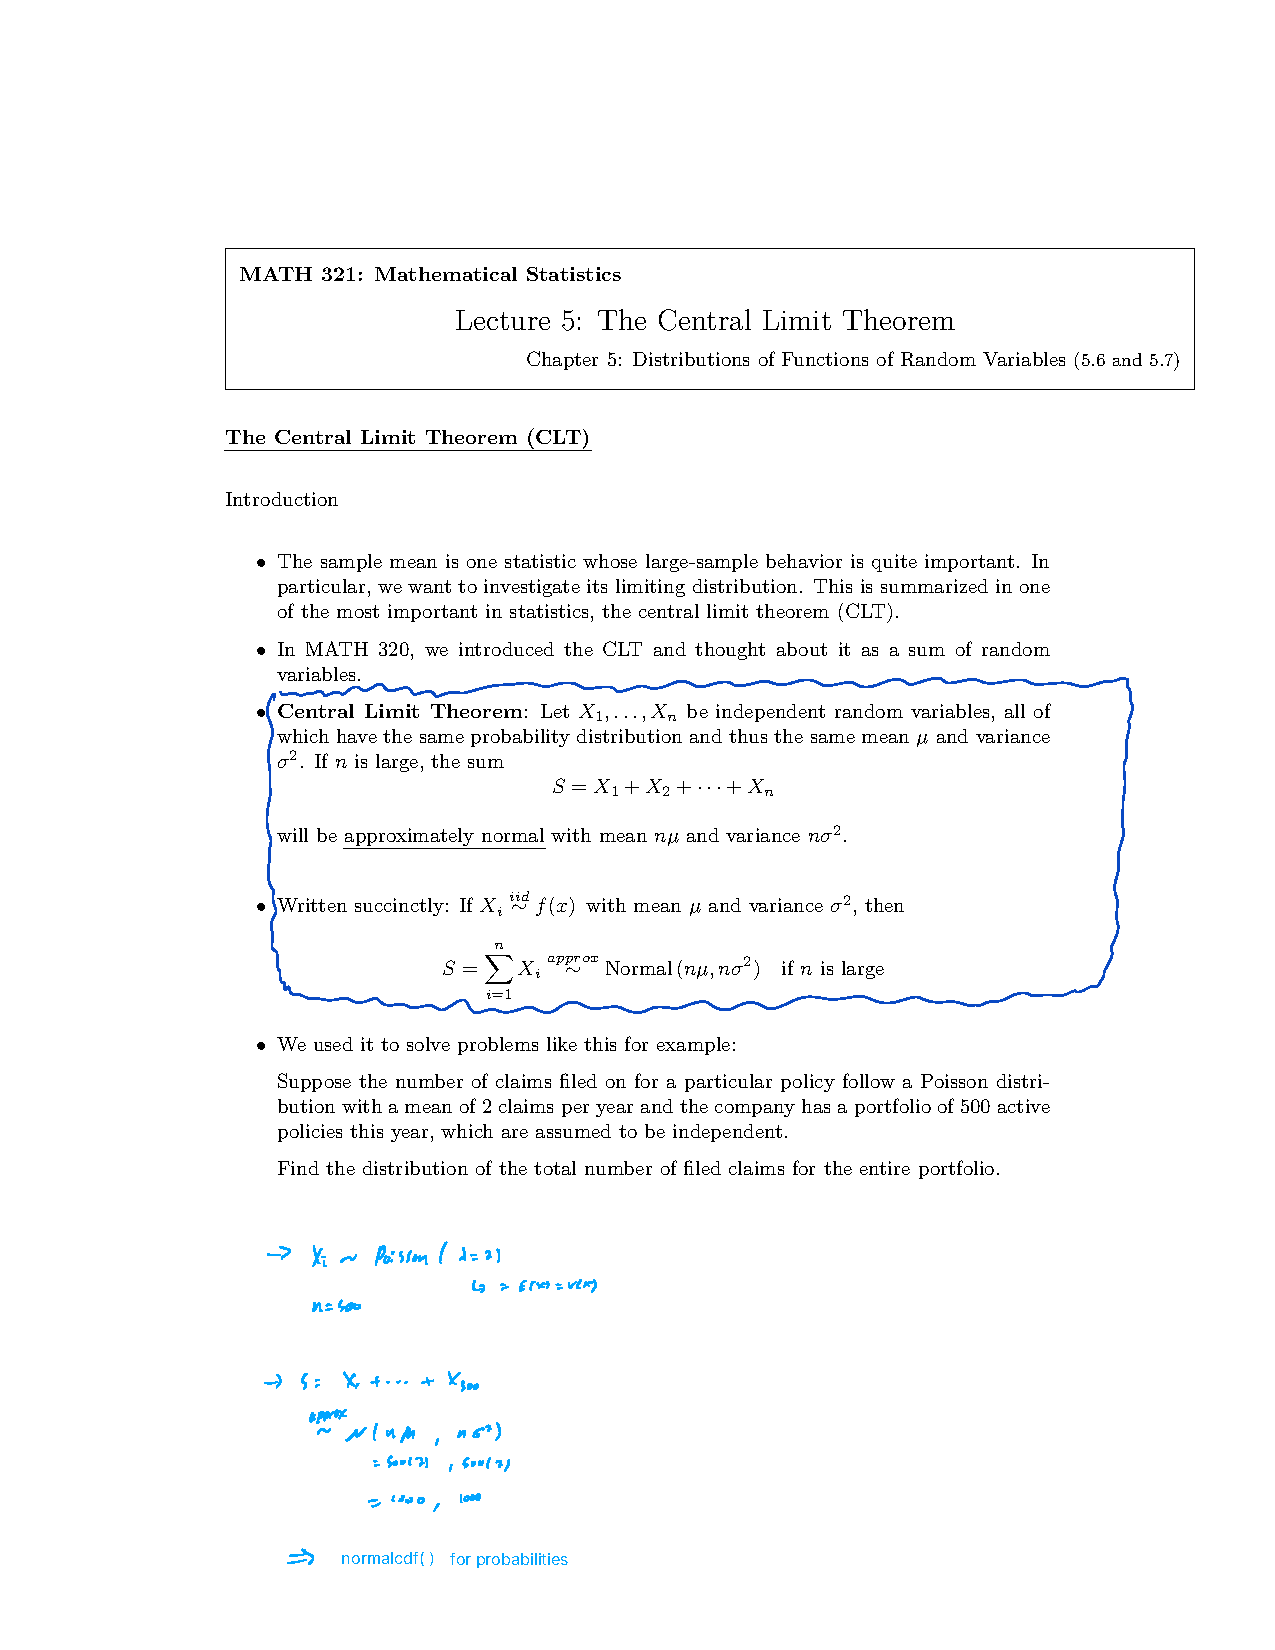
\includepdf[pages=-]{lecture-5-COMPLETED.pdf}\newpage
%----------------------------

%----------------------------
\subsection{Lecture 6 -- Confidence Intervals}
\includepdf[pages=-]{lecture-6-COMPLETED.pdf}\newpage
%----------------------------

%----------------------------
\subsection{Lecture 7 -- Hypothesis Tests}
\includepdf[pages=-]{lecture-7-COMPLETED.pdf}\newpage
%----------------------------


%-------------------------------------------------------------------------
\section{After Test 3}
%-------------------------------------------------------------------------

\secttoc

%----------------------------
\subsection{Lecture 8 -- Regression}
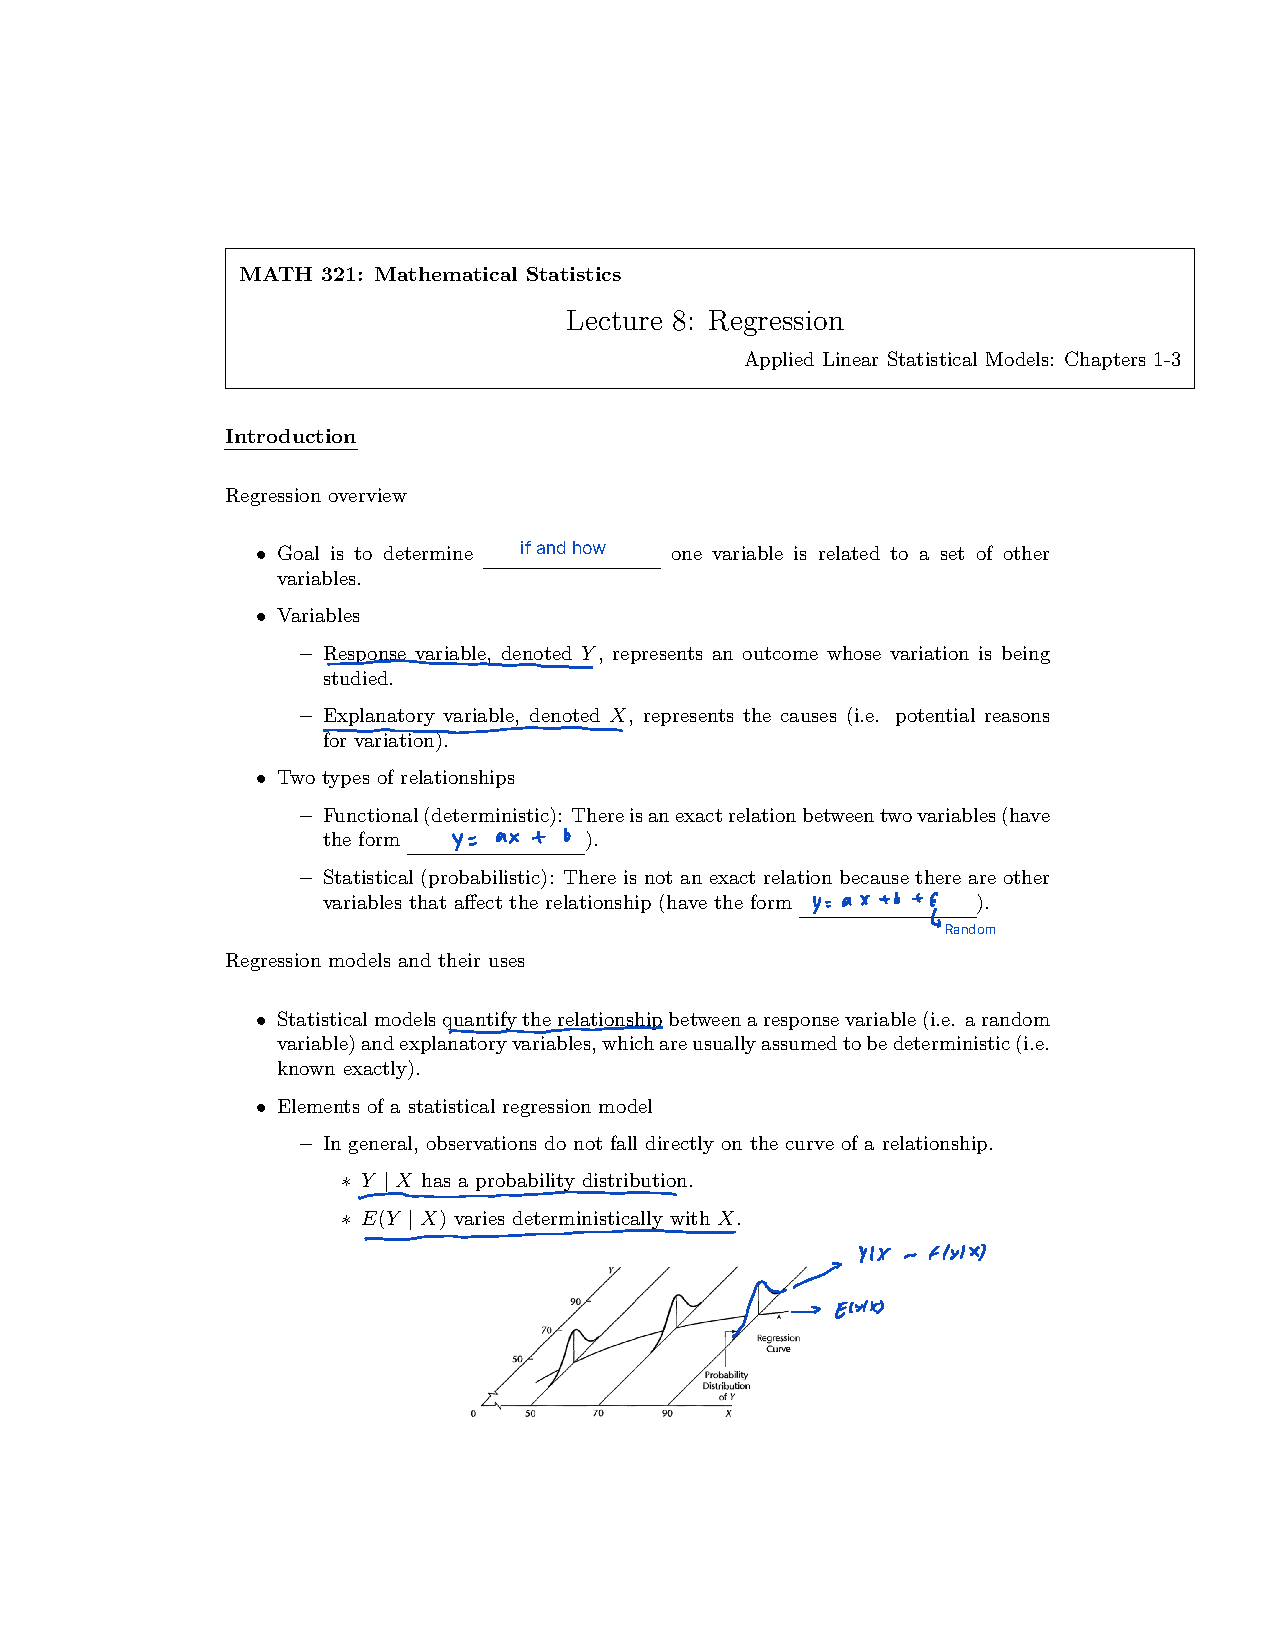
\includepdf[pages=-]{lecture-8-COMPLETED.pdf}\newpage
%----------------------------




\end{document}